\section{eBPF}\label{sec:ebpf_bg}
In 1992 a technology called `Berkeley Packet Filter' (BPF) was introduced into 
the Unix kernel.
By using BPF it is possible to attach a small BPF-program to some pre-defined hook points in 
the network stack of the kernel and filter packets there in a stateless manner.
This provided more efficiency since the packets did not need to be copied into 
userspace anymore but could directly be processed in the kernel.
One downside to such an approach however is that BPF-programs are limited by the 
so-called `BPF-verifier' which needs to check every BPF-program for safety e.g. 
to avoid infinite loops or access to invalid memory from withing kernel space. 
Today, the initial technology of BPF has evolved into `extended BPF' (eBPF) and 
allows for more versatile use cases.

\subsection{eBPF Hook Points}
The Linux kernel offers several hook points where eBPF-programs can be attached to.
Two main ones are one to attach eBPF-programs to the Traffic Control (TC) subsystem
and another one to attach them to the eXpress Data Path (XDP) subsystem.
The XDP hook, which is directly located in the NIC-driver, lies lower in the network 
stack than the TC-hook, which is located in the link-layer.
Despite being higher up in the network stack, the TC-hook has the big advantage that
it offers ingress and egress processing while the XDP-hook is available for ingress 
processing only.
This makes the XDP-hook suboptimal for the implementation of fast-relays since 
they heavily rely on processing packets at egress, after those were redirected
from ingress.
Figure~\ref{fig:ebpf-hooks} illustrates again the relative positions of the TC and
XDP hook points in the network stack.

\begin{figure}[htbp]
    \centering
    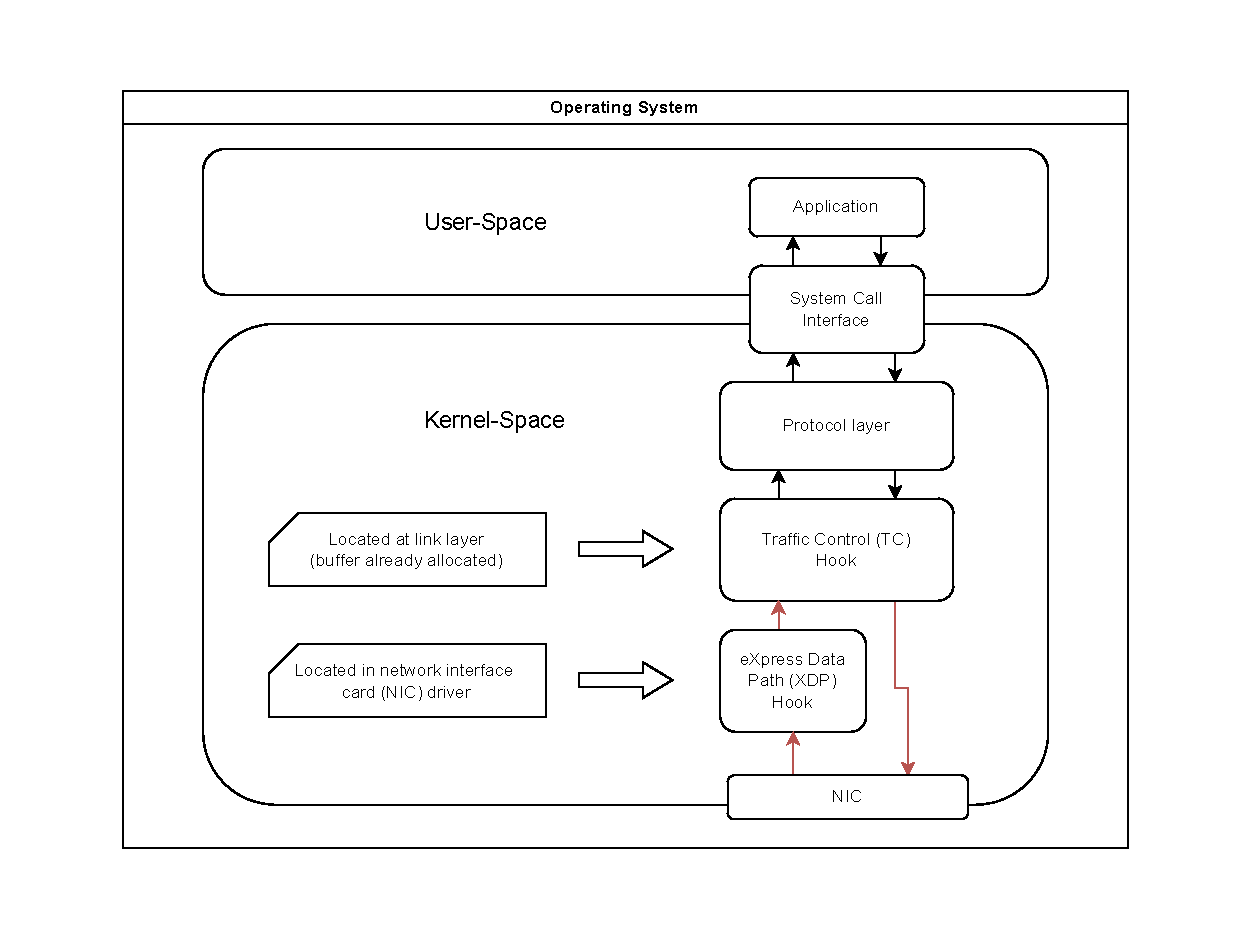
\includegraphics[width=\textwidth]{figures/02_background/ebpf-hooks.drawio.pdf}
    \caption{Abstracted view of Traffic Control (TC) and eXpress Data Path (XDP) hook points
    in the Linux kernel network stack.
    The red loop indicates the `short-cut' that is utilized by the fast relay.
    TC hook allows redirection directly to egress while XDP hook is only available
    for ingress processing.
    }\label{fig:ebpf-hooks}
\end{figure}

\subsection{Traffic Control Queuing Disciplines}
The Linux Traffic Control Subsystem uses Queuing Disciplines (qdiscs) to define how packets
are handled. TODO

\subsection{eBPF Verifier}
TODO

\subsection{Important eBPF Concepts}
TODO

\subsection{eBPF and Fast Relays}
TODO

\begin{figure}[htbp]
    \centering
    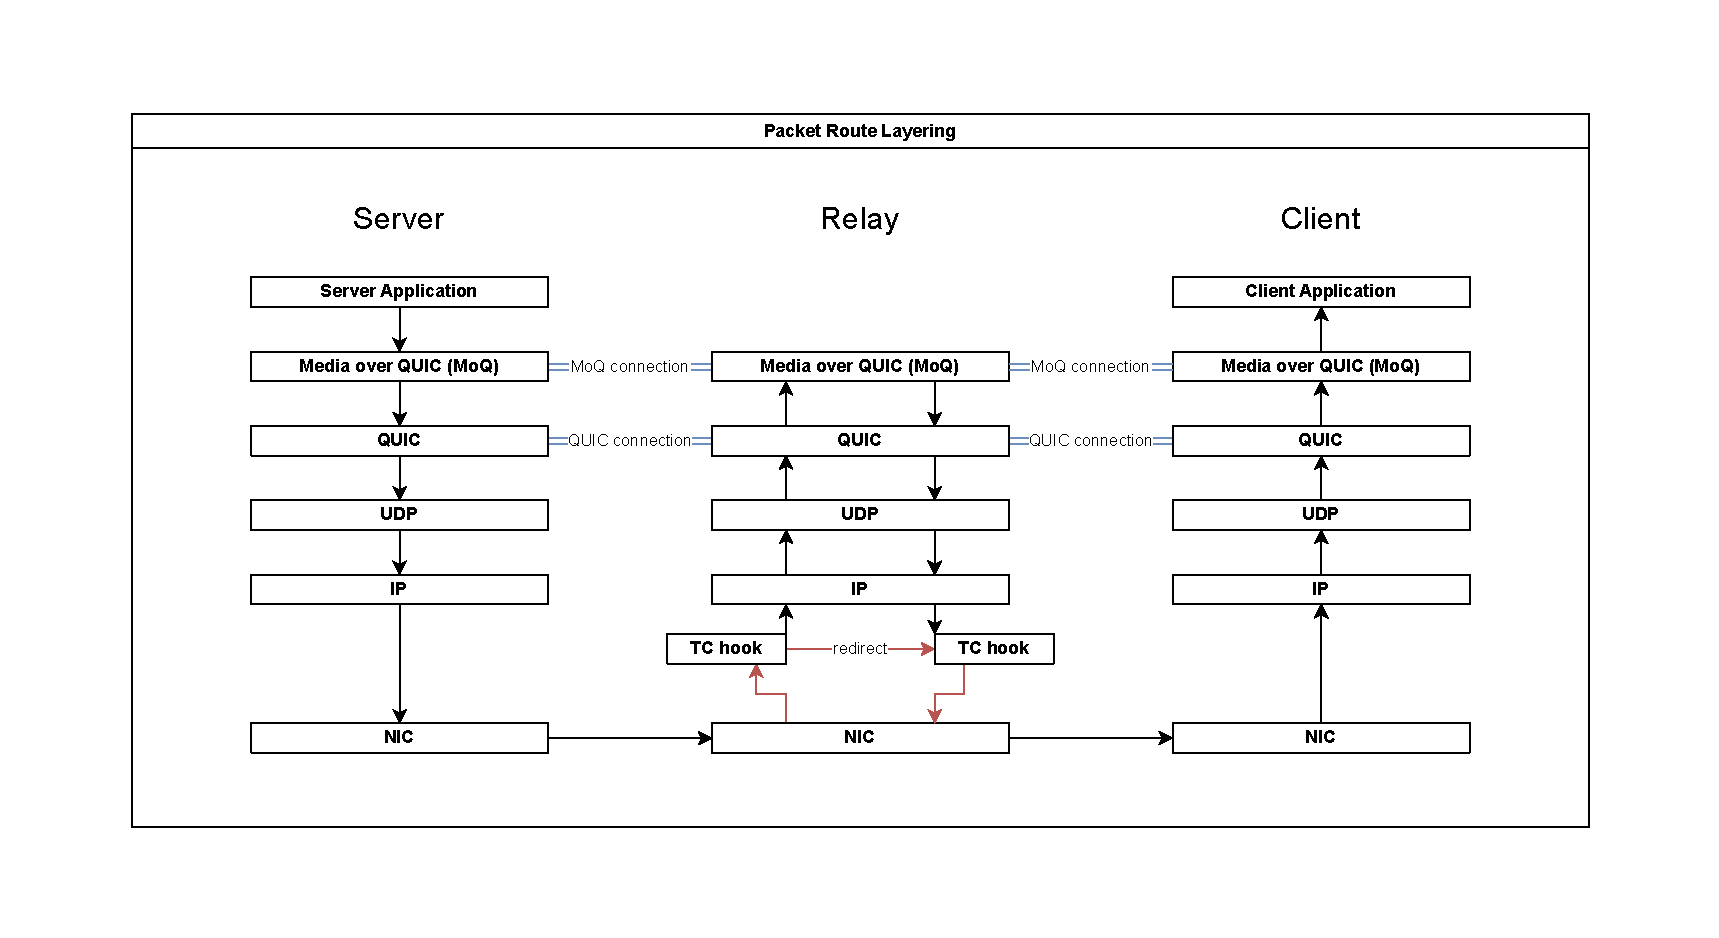
\includegraphics[width=\textwidth]{figures/02_background/route-layering.drawio.pdf}
    \caption{Conventional layers of a network stack for client, server and relay.
    The red loop indicates again the `short-cut' that is utilized by the fast relay and 
    based on eBPF packet-forwarding.
    This avoids the need for the packet to traverse the entire network stack of the relay 
    up to the userspace.}\label{fig:route-layering}
\end{figure}
